\documentclass[10pt,twoside,slovak,a4paper]{article}

\usepackage[slovak]{babel}
\usepackage[IL2]{fontenc} % lepšia sadzba písmena Ľ než v T1
\usepackage[utf8]{inputenc}
\usepackage{graphicx}
\usepackage{url} % príkaz \url na formátovanie URL
\usepackage{hyperref} % odkazy v texte budú aktívne (pri niektorých triedach dokumentov spôsobuje posun textu)
\usepackage{cite}

\raggedbottom % casti nebudu roztiahnute na celu vysku strany


\oddsidemargin=0cm % text na neparnych stranach bude vycentrovany lebo margin = 0
\evensidemargin=0cm
\textwidth=16.5cm % sirka textu na strane
\pagestyle{headings}

\title{Využitie statickej analýzy kódu pri vývoji softvéru
\thanks{Semestrálny projekt v predmete Metódy inžinierskej práce, ak. rok 2021/22, vedenie: Ing. Zuzana Špitálová}}

\author{Lukáš Častven\\[2pt]
	{\small Slovenská technická univerzita v Bratislave}\\
	{\small Fakulta informatiky a informačných technológií}\\
	{\small \texttt{xcastven@stuba.sk}}
	}

\date{\small  5. november 2021}

\begin{document}

\maketitle

\begin{abstract}
	Statická analýza je proces, pri ktorom je počítačový kód zanalyzovaný bez samotného spúšťania kódu.
	Po tejto procedúre sú programátorovi prezentované nájdené chyby, ich možný spôsob opravy a aj varovania
	o menej závažných nedostatkoch a ich riešenia. Pomocou tejto metódy dokážeme v celom analyzovanom projekte
	zlepšiť kvalitu kódu a udržať konzistentný štýl, ktorý taktiež spĺňa osvedčené postupy pri vývoji softvéru.
	Veľkou výhodou je tiež urýchlenie hľadania chýb a softvérových defektov v porovnaní s manuálnou kontrolou.
	V tomto článku pochopíme, prečo developeri používajú nástroje statickej analýzy, ako ich používajú
	na opravu a zlepšenie kódu a ako ich implementujú do ich pracovného prostredia.
\end{abstract}

\pagestyle{plain}

\section{Úvod}
S rastom komplexity vyvýjaného softvéru rastie aj jeho minimálna požadovaná kvalita. Chyby a defekty softvéru
dokážu firmám spôsobiť nemalé finančné straty. Existujú preto viaceré metódy ako kvalitu softvérových riešení zlepšiť
a udržať počas vývoja. Napríklad podrobné testovanie alebo revízie nového kódu iným developerom. V tomto článku si
bližšie priblížime metódu statickej analýzy, ktorá je používaná na odhalenie chýb a defektov a na udržovanie kvality
kódu na požadovanej úrovni.\cite{BrittanyJohnson,LisaNguyen}

O statickej analýze samotnej sa dozvieme v časti \ref{principy}, presnejšie, pochopíme čo to je (č.\ref{principy:co}) a
ako funguje (č.\ref{principy:ako}). Ako sa nástroje statickej analýzy používajú v praxi je uvedené v časti
\ref{vyuzitie}, kde zistíme ich benefity (č.\ref{vyuzitie:benefity}) a aj nedostatky (č.\ref{vyuzitie:nedostatky}).
Ako sú nástroje implementované v pracovnom prostredí je podrobnejšie vysvetlená v časti \ref{implementacia}. Ako s
nimi pracujú developeri v priebehu práce zitíme v časti \ref{dev}. A v neposlednom rade zistíme aké nové funkcionality
by chceli vývojari vidieť v budúconsti, časť \ref{navrhy}.


\section{Princípy statickej analýzy} \label{principy}
\subsection{Definícia statickej analýzy} \label{principy:co}
Statická analýza je proces, pri ktorom je kód posudzovaný bez spustenia samotného programu a bez vstupu. Preto sa
nazýva statická. Analyzuje sa zdrojový a v niektorých prípadoch aj objektový kód\footnote{Väčšinou ide o súbory s
	rozšírením nazvu „.o".}. Po úspešnom ohodnotení kódu, sú developerovi zobrazené nájdené chyby a defekty. Taktiež sú
poskytnuté vysvetlenia, prečo sú najdené chyby reálnymi chybami a ako ich je možné opraviť.\cite{wiki:Static_program_analysis}

\subsection{Funkcia statickej analýzy} \label{principy:ako}
Existuje veľa typov nástrojov statickej analýzy, ale nie všetky poskytujú rovnaké funkcionality ako iné. Našťastie
hlavný postup je jasne definovaný. Skladá sa len z dvoch krokov:

\begin{enumerate}
	\item Analýza zdrojového (objektového) kódu. \label{krok1}
	\item Informovanie o chybách, defektoch a narušení osvedčených postupov. \label{krok2}
\end{enumerate}

Aby sme lepšie pochopili, čo statická analýza robí, pozrieme sa na konkrétny nástroj FindBugs. Tento
nástroj sa používa na odhalenie chýb v programovacom jazyku Java.\cite{FindBugs}

Krok (\ref{krok1}) je za pomoci FindBugs realizovateľný buď cez plugin v integrovaných vývojarských prostrediach, alebo
cez príkazový riadok. Po zanalyzovanií kódu, FindBugs rozdelí defekty do kategórií podľa ich závažnosti. Tie sú:
vysoká, stredná a nízka. Následovne, ako súčasť kroku (\ref{krok2}), poskytne vývojarovi aj niekoľko možných návrhov
rýchlych opráv\footnote{ang. Quick fixes}.\cite{BrittanyJohnson,NathanAyewah}


\section{Využitie pri vývoji softvéru} \label{vyuzitie}
V praxi nie je využitie statickej analýzy bezproblémové. Samozrejme, benefity tejto metódy sú jasne viditeľne, avšak
developerov viac odrádzajú tažkosti a nedostatky ako pozitívá, ktoré táto metóda poskytuje. V tejto časti si
rozoberieme vedeckú prácu \textbf{Why don't software developers use static analysis tools to find bugs?}\cite{BrittanyJohnson}
a zistíme prečo je predošlé tvrdenie pravdivé.

V tomto príspevku autori uskutočnili rozhovory s dvadsiatimi vývojarmi na tému statická analýza. Zozbierané odpovede
zkategorizovali do niekoľkých okruhov a rozdelili na pozitívne a negatívne.

\subsection{Benefity} \label{vyuzitie:benefity}
\subsubsection*{Automatické hľadanie chýb}
5 z 20 účastníkov tejto práce si myslí, že nástroje statickej analýzy sa oplatí používať práve z tohto dôvodu.
Manuálna kontrola je zdĺhavá a namáhavá, oproti automatickej statickej analýze.

\emph{„Hoci čo, čo zautomatizuje nudnú prácu je skvele."}

\subsubsection*{Pred-integrované v prostredí}
Ako dôvod prečo využívajú statickú analýzu, zvolili 3 účastníci pred-integráciu v ich pracovnom prostredí. Veľa
integrovaných vývojových prostredí už má v sebe zabudované tieto nástroje, aj keď ide iba o ľahké verzie, ktoré nevedia
odhaliť všetky chyby.

\subsubsection*{Udržiavanie tímových praktík}
Zvýšenie povedomia o možných problémoch, alebo o chybách z nepozornosti skôr vo vývojovom cykle je kľúčové ku udržaniu
tímoveho vývojového úsilia. Taktiež sa ľahšie udržuje jednotný štýl kódu. 7 z 20 developerov označili tento benefit ako
rozhodujúci v otázke prečo používajú statickú analýzu.

\subsubsection*{Komunikácia}
Nástroje statickej analýzy sú užitičné pri komunikácií a pri presadzovaní štandardov a štýlov vo vývojovom tíme,
uviedli 2 respondenti.

\subsubsection*{Nastaviteľnosť}
3 účastníci využívajú nástroje statickej analýzy pre ich schopnosť vytvorenia vlastných typov chýb, čo im umožňuje
automatické detekovanie chýb, ktoré sú špecifické pre daný projekt.

\subsection{Nedostatky} \label{vyuzitie:nedostatky}
\subsubsection*{Výsledok analýzy}
Až 14 z 20 respondentov označilo zlý výstup a úbohú prezentáciu ako dôvod, ktorý ich odrádil od určitého nástroja
statickej analýzy.

Je známe, že tieto nástroje produkujú aj falošné pozitíva, čiže hlásenia o chybách, ktoré nie sú
naozajsnými chybami. Ak nástroj produkuje viac falošných pozitív ako reálnych pozitív, uživateľ musí manualné
prefiltrovať všetky a zistiť, čo je správne. Toto daného uživateľa demotivuje, čo spôsobí vymenenie nástroja, alebo v
horšom prípade, celkové vynechanie statickej analýzy.

V masívnejších projektoch je počet defektov veľký a ak prezentácia je neprehľadná a nečitateľná, developer sa ľahko
stratí v kvantách informácií. To znamená, že viac času je minutého na opätovné zorientovanie sa, ako na samotné
opravenie chýb a toto, ako v predošlom odseku, môže viesť k vynechaniu statickej analýzy kompletne.

\subsubsection*{Tímová práca}
Vývoj softvéru je prevažne tímová práca, preto je dôležité, aby inžinieri nástrojov statickej anaýzy brali tento
dôležitý fakt do úvahy pri ich vytváraní. Jeden vývojar uviedol, že síce sú tieto nástroje užitočné, ale neexistuje
jednoduchý spôsob ako zdielať nastavenia v tíme. Z tohto úkonu sa takto stáva nepraktický manuálny proces nastavovania,
ktorý v prípade zmeny štandardov a nastavení zapríčiní zmätok a chaos.

Viacerí respondenti by chceli aby tieto nástroje zjednodušili komunikáciu a kolaboráciu v tíme. Aby nemuseli narušiť
svoj pracovný priebeh.

Spolu označilo túto kategóriu 9 z 20 opýtaných ako závažný problém.

\subsubsection*{Netriviálna nastaviteľnosť}
Každý projekt je inakší, ma iné požiadavky, restrikcie a kvality. Preto je nastaviteľnosť dôležitý aspekt pre využívaný
nástroj. Ale ako uviedlo 17 z 20 developerov, táto vlastnosť je silne netriviálna alebo nespĺňa vývojarove predstavy.

Vývojar potrebuje niekoľko hodín len na to aby sa naučil ako nastaviť daný nástroj. \emph{„Mnohe nástroje sú tak ťažko nastaviteľné, že vám v tom rovno zabránia."}

Problém, ktorý mala väčšina respondentov, je nemožnosť dočasne vypnúť upozornenia na špecifický typ defektov. Niektoré
nástroje poskytuju vypnutie natrvalo, ale toto sa zas nepáči developerom, lebo nikto nevie vopred povedať, či daná,
teraz ignorovateľná chyba, bude taká aj v budúcnosti.

\subsubsection*{Nejasnosť}
Väčšina developerov nedostatočne využíva túto metódu pre nejasnosť vo výstupe. Neschopnosť porozumieť nájdeným chybám
je pre 19 z 20 vývojarov bariera. Nezrozumiteľné a nevyužiteľné vysvetlenia alebo málo poskytnutých informácií sú hlavné
faktory vzniku nejasností.

Najčastejšie spomínaný problém je nedostačujúca alebo neefektívna implementácia rýchlych návrhov opráv. Väčšina z
respondentov by prijala návrhy počas opravovania nájdených chýb. \emph{„Ak mi dokážeš povedať o chybe, tak by si mi mal
	vedieť aj povedať ako ju opraviť."}, vyhlásil jeden z respondentov.

\section{Implementácia nástrojov statickej analýzy} \label{implementacia}
Existuje viacero typov nástrojov statickej analýzy. Nástroje implementované v integrovaných vývojových prostrediach (IDE),
ktoré bežia v pozadí, poskytujú instantú spätnú väzbu počas práce, avšak tento typ nachádza len jednoduché chyby nie
komputačne náročné na odhalenie.

Niektorí developeri nepoužívajú IDE, vtedy prichádza do úvahy nástroj integrovaný do
kompilátora daného programovacieho jazyka.

A v neposlednom rade poznáme aj rigorózne analyzátory, ktoré sa väčšinou
spúšťajú cez noc, lebo dlho a podrobne analyzujú daný kód.\cite{BrittanyJohnson, LisaNguyen}

\section{Využitie v praxi} \label{dev}
Samozrejme dôležitá je prax, to ako uživateľ používa a vníma daný nástroj\cite{LisaNguyen}.
Diagram Obr. \ref{diagram} znázorňuje ako sú nástroje statickej analýzy používané v praxi.

\subsection*{Kedy sú používané}
Developeri využívajú tieto nástroje behom voľna (v časoch medzi stretnutiami, alebo keď majú časové okno). Opravovanie
nájdených chýb je v priemere vykonávané v úsekoch od 10 do 30 minút a oprava jedného nálezu zaberie zhruba menej ako 1 deň.

\subsection*{Ciele pri používaní}
Zvyčajne je vývojarovým cieľom opraviť všetky defekty alebo ich opraviť čo najviac v stanovenom časovom úseku. Preto
je čas hlavný dôvod ukončenia opravy a toto priamo ovplyvňuje aké chyby si developer vyberie na opravu.

\subsection*{Výber chýb na opravu}
Developer si prevažne vyberie chybu, ktorú vie opraviť, má na to znalosti o celkovom projekte alebo má skúsenosť s
daným nástrojom statickej analýzy. Pri varovaniach na nedostatky, ktoré ale nie sú chyby, však dominuje skúsenosť
s nástrojom. Preto je dôležité aby dizajn daného nástroja podporoval správanie, ktoré vedie k oprave, aj keď vývojar
nedokáže chybu opraviť.



\begin{figure*}[tbh]
	\centering
	\caption{Práca so statickou analýzou v praxi.}
	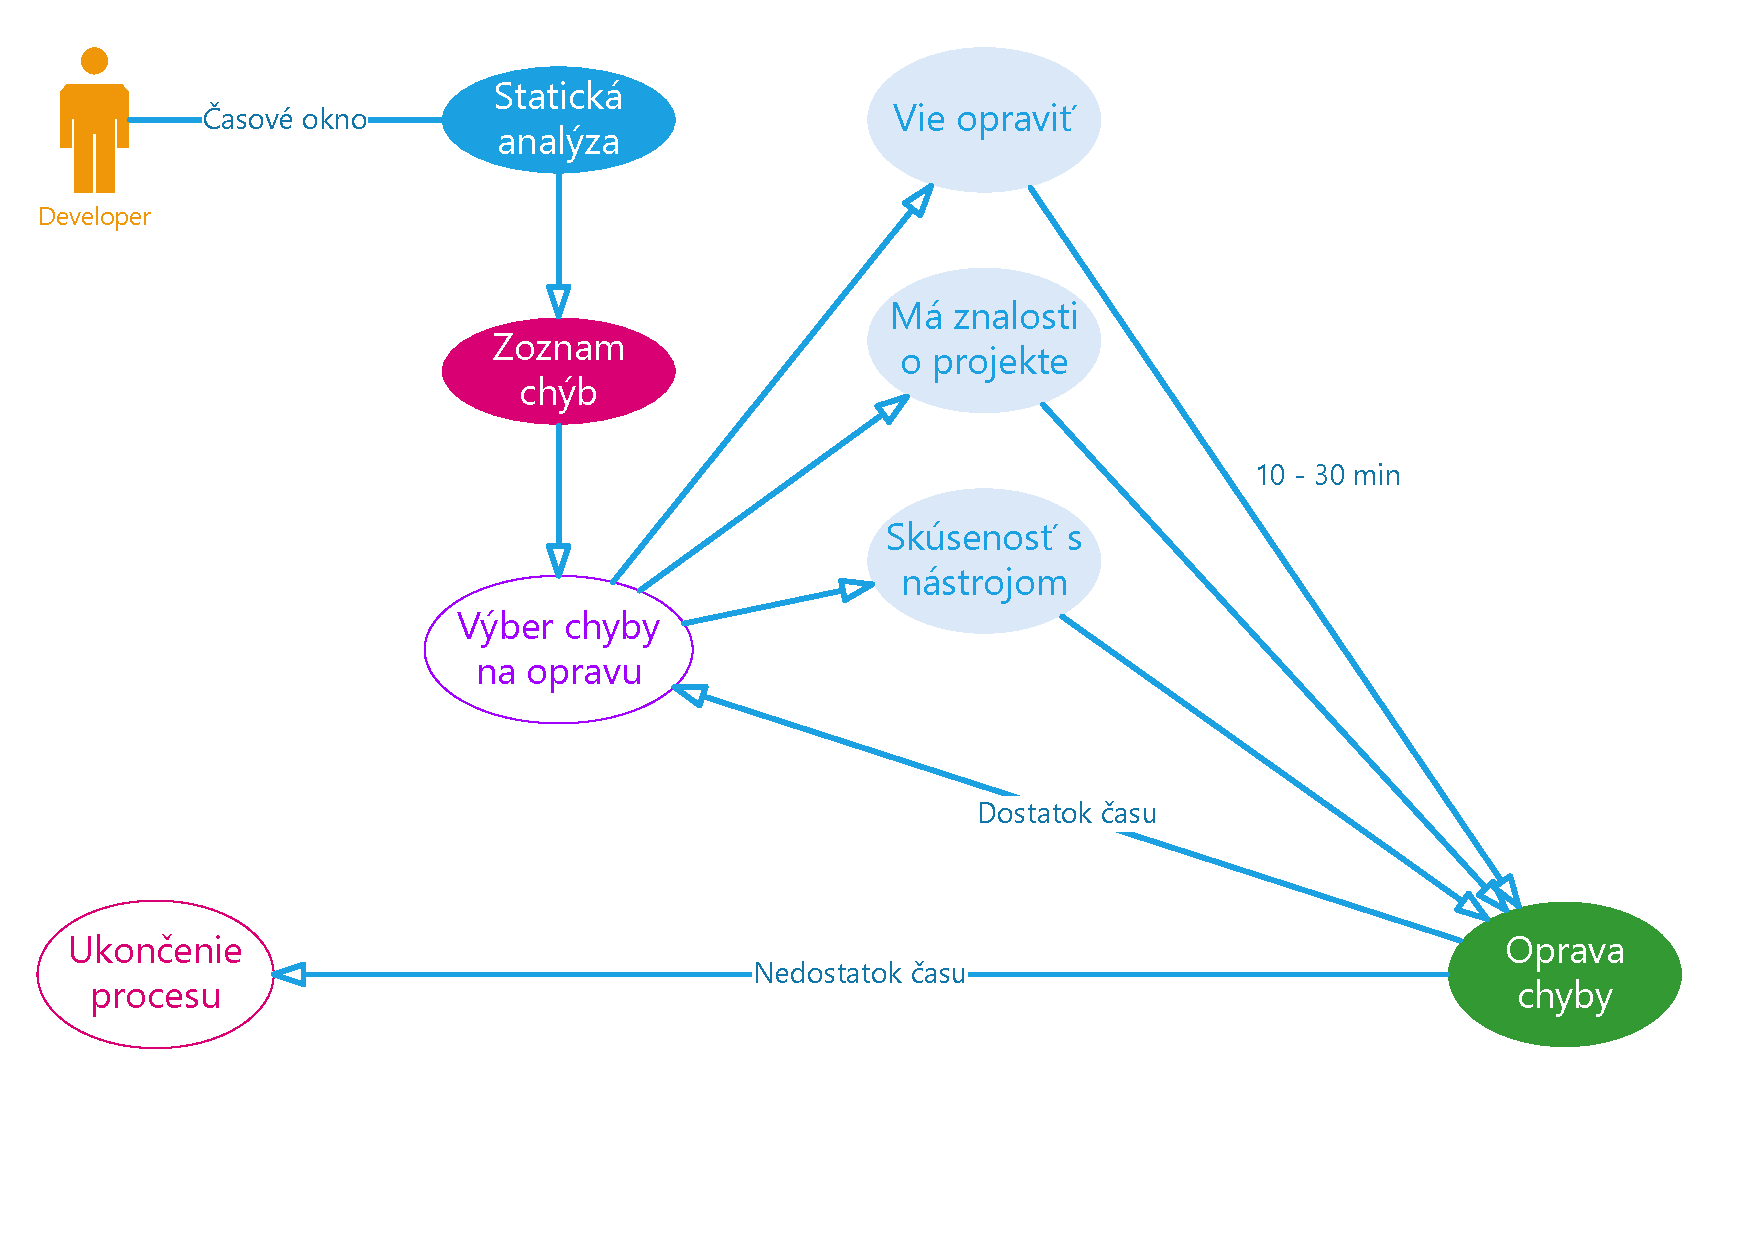
\includegraphics[scale=0.50]{vyuzitie.pdf}
	\label{diagram}
\end{figure*}


\section{Návrhy na zlepšenie} \label{navrhy}
Najvyužívanejšie funkcionality sa týkajú opravy chýb. Návrhy rýchlych opráv by mali ukázať porovnanie terajšieho kódu a
kódu po aplikovaní návrhu. Taktiež by sa developerom páčila možnosť aplikovania opravy rovno z nástroja. Táto aplikácia
by mala mať viacero možností, aplikovanie celého návrhu, iba časti, alebo vôbec.

Samotné zobrazenie chýb má tiež zopár aspektov na vylepšenie. Malo by byť čo najrýchlejšie, aby nenarušovalo pracovný
priebeh, čiže najlepšie vyhodnocované v pozadí s okamžitou spätnou väzbou. A malo by aj uľahčiť kolaboráciu a
komunikáciu. Napríklad posielanie správ alebo zdielanie nálezou s inými.

Nakoniec developeri by preferovali aj iné formy výstupu ako len list s chybami. Grafy, diagramy alebo teplotné mapy
s modulmi kódu ako nódami.\cite{BrittanyJohnson,LisaNguyen}


\section{Záver}
Statická analýza pomáha developerom zlepšiť a udržať kvalitu kódu v projektoch. Dokáže násjť chyby urobené z
nepozornosti, bezpečnostné defekty, nedodržiavanie osvedčených postupov, narušenie štýlu a mnohé iné nedostatky.

Aj keď v teórií prináša statická analýza veľa pozitív, v praxi nie je práca s nástrojmi statickej analýzy
bezproblémová, to zapríčiňuje nedostatočné využívanie. Chyby v implementácií tejto metódy do pracovných prostredí
vývojarov prevážia jej benefity.

Preto by mali inžinieri statickej analýzy viac počúvať spatnú väzbu k ich nástroju od uživateľov a rozvíjať
funkcionality v tomto smere.

\section*{Reakcia na prednášky}
\paragraph{Spoločenské súvislosti.}
Každým dňom sa naša spoločnosť spolieha viac a viac na softvérové riešenia, či už v medicíne pri záchrane životov,
vo finančnom sektore a napríklad aj v doprave. To zapríčiňuje rast minimálnej kvality vyvýjaného softvéru, lebo aj
tá najmenšia chyba, napríklad v medicíne, mohla spôsobiť smrť. Preto veľa IT tímov používa nástroje statickej analýzy.
Tie dajú developerovi viac času na riešenie dôležitých chýb a defektov, čím sa zdvíha úroveň finálneho softvérového
riešenia.

\paragraph{Historické súvislosti.}
V sedemdesiatych rokoch minulého storočia boli nízko levelové jazyky široko rozšírené. Avšak v týchto jazykoch
bolo veľmi ľahké urobiť chybu z nepozornosti. Toto motivovalo Stephena Johnsona pri výrobe prvého nástroja statickej
analýzy. Navrhol ho počas jeho práce v Bell Labs a nazval ho Lint. Tento nástroj, spolu aj s postupom ako rozdeliť
vývoj na čisto programovanie a potom na retroaktívne hľadanie chýb s pomocou Lintu.~\cite{Lint}

\paragraph{Technológia a ľudia.}
Vďaka statickej analýze je kvalita kódu počas celého vývojového cyklu udržovaná na predom stanovenej úrovni. Toto je
zapríčinené viacerými benefitami, ako napríklad automatické hľadanie chýb a defektov a udržovanie konzistentného
štýlu kódu v celom projekte. Avšak implementácie nástrojov nie sú dokonalé a majú určité nedostatky, ktoré
dokážu uživateľa demotivovať a to môže zapríčiniť vynechanie statickej analýzy počas vývojového cyklu. Našťastie,
inžinieri týchto nástrojov dávajú veľký dôraz na spätnú väzbu od developerov a na jej základe sa snažia napraviť a
vylepšiť ich nástroje. A tým celkovo posúvaju obor statickej analýzy vpred.

\paragraph{Udržateľnosť a etika.}
Udržateľnosť je jedna z najdôležitejších vlastností dlhodobých IT projektov. Statická analýza priamo podporuje
udržatelnosť softvérových riešení, tým že poskytuje IT tímom mnohé benefity, medzi ktoré patria napríklad automatické
hľadanie chýb alebo dodržiavanie štandardných štýlov kódu v celom projekte. A taktiež napomáha developerovi pri
dodržovaní určitých bodov etického kódexu (Software Engineering Code of Ethics and Professional Practice).

\bibliography{literatura}
\bibliographystyle{ieeetr}


\end{document}
